\chapter[Extending the Password Space with Emojis]{Extending the Password Space with Emojis}\label{chap:emojipasswords}
%TODO mehr ``human factors'' statt ``usability''
%Lingo: Visual memory vs lexical memory
% ultimate goal: decide on recommendations of emoji-pws, understand the consequences and constraints, and ensure first-movers don't trip over wires.
%in chapter \ref{chap:pws_and_personality} we found that certain users are more open to a passwords that contain emojis. We had introduced this policy as a novel, sort of provoking policy to trigger reactions to a new situation. only a few attitudinal aspects evaluated. now it is time to explore their feasibility. 

Our previous efforts to support users focused on suggestions, feedback, and feed-forward to help users create stronger passwords. We now continue to explore a different dimension of persuasive design that was supposed to make it easier for users to create both strong and highly memorable passwords. To that end, we looked at \textbf{emojis} as possible solution, since we have found positive attitudes towards using them inside passwords (see Chapter \ref{chap:pws_and_personality}). Emojis are \textit{pictographs} used to express emotions or communicate words with pictures. The Unicode consortium has made them part of the de-facto digital encoding standard\footnote{\label{foot:emoji-standard}\url{http://www.unicode.org/reports/tr51/}\la{10.03.2018}}, which led to widespread adoption very quickly. In 2015, the ``face with tears of joy'' emoji (\emoji{1F602}) became the Oxford dictionary's \textit{word of the year}\footurl{http://blog.oxforddictionaries.com/2015/11/word-of-the-year-2015-emoji/}{10.03.2018}, which shows the cultural impact of these colorful symbols. A recent report claims that roughly three quarters of Internet users communicate with emojis on a regular basis \cite{EmogiResearch2016}. While image-based passwords were proposed decades ago (see Section \ref{sec:rw:graphical_pws}), the recent success of emojis has given graphical authentication new momentum. 

Emojis are an opportunity to increase security, because they can add more complexity to passwords. Adding an emoji to a weak password like \texttt{iloveyou} could already make it less predictable, e.g. \texttt{iloveyou\emoji{1F981}}. We have also seen that users' mental models are built around complexity, and not necessarily around length. Thus, an emoji-password like \texttt{Corr3ct\emoji{1F434}\emoji{1F50B}\emoji{1F4CE}} might be perceived as more secure than the original passphrase. Past studies have also shown that graphical authentication can benefit from the \textit{picture superiority effect}. Hence, using emojis inside passwords might have usability advantages, and we also see them as an \textbf{enabling technology} that empowers users to pick more creative and memorable secrets, i.e., a persuasive design strategy. At the same time, existing authentication back-ends do not require significant changes to make emoji-passwords work. Since emojis are encoded as regular characters, the only potential change is to use a different version of UTF. Theoretically, 90\% of web-pages are compatible with emojis in password fields already now (see Footnote \ref{foot:emoji-standard}). Consequently, some service providers have started to allow emojis as part of user-chosen passwords also on the back-end. Twitter, Slack and StackOverflow are among these pioneers. 

However, the adoption comes with certain risks. Emojis are primarily used on mobile devices \cite{EmogiResearch2016}. Hence, adding emojis to passwords on a smartphone is easy, but there might be problems when the user tries to enter their emoji-password on a desktop: Typical input solutions possible with \textit{software} keyboards get left out on the desktop. Some applications have enabled indirect emoji input through the mouse in a graphical user interface, so it is not impossible to enter an emoji-password across different platforms. On the other hand, the specific images used to render emojis are platform-dependent: a bird emoji on a native iOS soft-keyboard looks different on Android (see Figure \ref{fig:emojipasswords:emoji-bird-comparison}). This \textit{fragmentation}\footurl{https://blog.emojipedia.org/2018-the-year-of-emoji-convergence/}{16.02.2018} introduces new issues not typically found with other graphical authentication schemes, where there is more control over the images. 
% GOAL
Thus, we wanted to understand the usability factors and constraints of emoji-passwords to gauge the feasibility of this authentication mechanism.

\begin{figure}
	\centering
	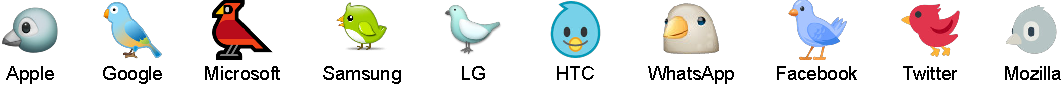
\includegraphics[width=\linewidth]{figures/emojipasswords/emoji-bird-comparison}
	\caption{
		\label{fig:emojipasswords:emoji-bird-comparison}
		Although the ``bird'' emoji is encoded with the same unicode character (U+1F426), its visual representation differs strongly across platforms and vendors. This has specific ramifications on the use of emojis inside passwords, which we address in this project.
	}
\end{figure}

%QUESTIONS
In this chapter we explore pragmatic and hedonic qualities of emoji-passwords. We aim to answer the following research questions:
\begin{itemize}
	\item[RQ1] Do emojis in passwords help users create more \textbf{memorable} passwords?
	\item[RQ2] How do platform-dependent renderings (\textbf{fragmentation}) affect memorability?
	\item[RQ3] What is the most feasible \textbf{user interface} to enter emoji-passwords?
	\item[RQ4] What are users' password \textbf{selection strategies} and behaviors?
	\item[RQ5] What are users' general \textbf{attitudes} towards using emojis inside passwords?
\end{itemize}

This chapter reports on a mixed-method experiment carried out to investigate the usability of alphanumeric passwords that contain emojis. In the following, we put the design space for emoji-passwords into context, describe an empirical research study, and derive implications on the effective use of emoji-passwords.

\fbox{
	\hspace{0.2cm}
	\parbox[c][8cm]{0.95\linewidth}{
		\subsection*{Publication Statement}
		Beside myself, Florian Mathis and Heinrich Hussmann made contributions to the project. The results of the study were published at OzCHI 2017 \cite{Seitz2017Emojipasswords}. The chapter elaborates on the results of that paper and provides significant additional analyses:
		\begin{itemize}[leftmargin=*]
			\item We show a detailed quantitative breakdown of selection strategies, in particular regarding the position of the emojis and relations to the passwords.
			\item We take a deep-dive into successful and unsuccessful authentication events in the second part of the study. 
			\item We provide new thoughts on the ramifications of using emojis inside alphanumeric passwords.
		\end{itemize}
	}
	\hspace{0.2cm}
}


\section{Background and Context}
\subsection{Emojis}
%definition and history / origin
Literally translated from Japanese, emojis\footnote{The plural form for ``emoji'' is both ``emoji'' (Japanese) and ``emojis'' (adopted to English). For clarity reasons the chapter sticks to ``emoji\textbf{s}''.} are ``picture words'' \cite{Taggart2015NewWords}. They are primarily used in mobile messaging applications like WhatsApp, iMessage, and alike, to express emotions and add subtext in messages. Before emojis arrived, this has been possible with \textit{emoticons}, i.e. combinations of regular characters that convey emotions like \texttt{:-)} \texttt{<3} and \texttt{:-O}. However, emojis are visually richer and much more versatile. The current version of the Unicode standard lists around 2800 emojis (see Footnote \ref{foot:full-list-of-emojis}) categorized by topics, and roughly 150 are added each year. In 2015, emojis saw a stark increase in usage numbers. Both iOS and Android added special software keyboards that allowed users to easily enter emojis through direct touch input. %This contributed to the addition of emojis in half the image-captions on Instagram\footurl{https://engineering.instagram.com/emojineering-part-1-machine-learning-for-
%emoji-trendsmachine-learning-for-emoji-trends-7f5f9cb979ad}{10.03.2018}. 
Often, users replace entire words or blocks of text with emojis. Although emojis are useful to overcome language barriers, their meaning is not always clear \cite{Miller2015BlissfullyHappyEmoji,Tigwell2016EmojiMisunderstandings}. Researchers have started to investigate misinterpretation in many ways, and have proposed solutions like a ``disambiguation API'' \cite{Wijeratne2010}. 

\subsection{Emojis in Authentication}
% visual authentication
The growing adoption rates of emojis in various application areas has not gone unnoticed by the \gls{USEC} community, who started trying to improve authentication schemes with emojis. One of the first solutions was presented by Intelligent Environments\footurl{https://www.intelligentenvironments.com/now-you-can-log-into-your-bank-using-emoji/}{10.03.2018}. Their \textit{emoji-passcode} system would allow customers to select four emojis from a 9x5 grid to log into mobile banking apps. However, the concept has not been widely adopted. Golla \etal, respectively Kraus \etal, proposed a similar system that was targeted at screen-locks for mobiles \cite{Golla2017EmojiAuth, Kraus2017Emoji}. In essence, their EmojiAuth system replaces each digit on a PIN-pad with an emoji. In two user studies, they evaluated the concept and showed that both security and usability of unlock mechanisms can be improved this way. On the other hand, we were able to find only one publication about using emojis as part of an alphanumeric password  \cite{AlHusainy2015EmojiPasswords}. Al-Husainy and Mali focused on user-account passwords on desktop computers but did not present an empirical evaluation of the concept. We believe web pages and mobile applications are the primary use case for emoji-based authentication. This application area is still underexplored. 

\subsection{Research Opportunities}
The combination of emojis and alphanumeric characters generates a wide range of research questions, and we can only answer a small subset of them. In particular, we explore password selection strategies that may hint at potentially risky behavior. It is likely that emoji-passwords share some traits of alphanumeric passwords. For instance, the topology of a password is an important metric to gauge its guessability. Therefore, we would expect to observe some topologies reported by Weir \etal  \cite{Weir2010MetricsPolicies}, Ur \etal \cite{Ur2015PWCreationLab}, and Kuo \etal \cite{Kuo2006HumanSelectionMnemonic}. The latter indicated that some users had already used emoticons inside passwords in 2005. Although we cannot realistically measure guessability of emoji-passwords at this time, we can explore emerging patterns. For instance, we can elicit where users put their emoji and how they choose it. Emoji-passwords are a hybrid between knowledge- and recognition-based authentication, so they demand effort from both the lexical and visual memory \cite{Renaud2009VisualSnakeOil}. Therefore, this approach could turn out to be either a memorability advantage or disadvantage. Since the answer to this question is very open, we refrain from generating hypotheses altogether.

%TODO: this paragraph does not make tooooo much sense, but is intended to show a) many unanswered questions, b) what we expect to find (but that's not enough to form hypotheses), c) that we can already discover patterns that serve modelling password strength/weaknesses.

%Finding the right emoji:
%\cite{Pohl2017BeyondTextEmoji} input problems
%Other use of emojis in research: 
%\cite{Marengo2017EmojiPersonality} using emoijs as indicators for personality
%\cite{Lorenzi2017Emojitcha} using emojis as captchas

\section{User Study}
% GOALS
The goal of our project was to understand the human factors and usability constraints of emoji-passwords, which can be used to evaluate the idea of empowering users as persuasive strategy. To achieve this goal, we created a prototype that allowed entering emojis inside password-fields and evaluated it with a mixed-methods user study to cover a large spectrum of opportunities and caveats. The first part took place in a controlled lab environment, while the second was carried out remotely without moderation. To explore different dimensions of usability and to follow common practice, password selection and recall were spread out across different days. In the following we describe the prototype, the procedure of the two methods, the corresponding variables, and the sample of our study. 

% overview + motivation to use mixed methods.
\subsection{Prototype}
\begin{figure}
	\centering
	\begin{subfigure}[t]{0.45\textwidth}
		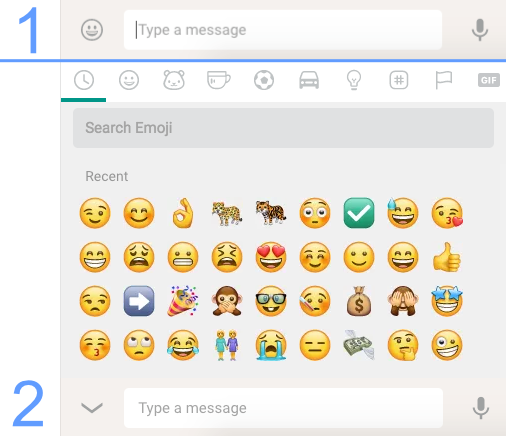
\includegraphics[width=\textwidth]{emojipasswords/whatsapp-picker-steps}
		\caption{\label{fig:emojipasswords:whatsapp-point-and-click}Two-step point-and-click interface  in WhatsApp.}
	\end{subfigure}
	\hspace*{0.1cm}
	\begin{subfigure}[t]{0.45\textwidth}
		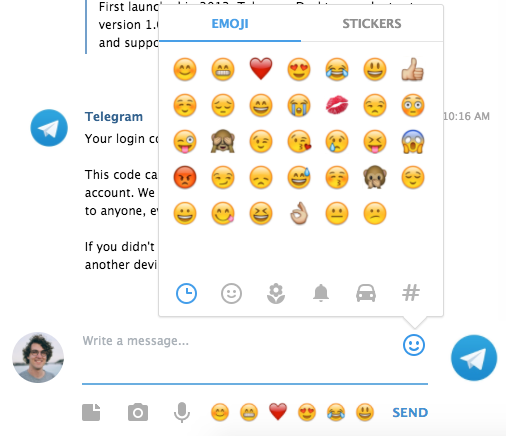
\includegraphics[width=\textwidth]{emojipasswords/telegram-picker}
		\caption{\label{fig:emojipasswords:telegram-point-and-click} Telegram shows the picker after the user hovers  the emoji button. Moreover, recently used emojis are shown beneath the text-field.}
	\end{subfigure}
	
	\caption{\label{fig:emojipasswords:real-world-pickers}
		Examples for point-and-click interfaces (``emoji picker''). \textit{Progressive disclosure} is used to access
		the list of available emojis: The user first needs to interact with a control element (emoji button) or start typing a special character (mostly ``:''), before an emoji can be selected by clicking or auto-completion of the shortcode. The emoji is then inserted into the text field.
	} 
\end{figure}
% general ways to do this.
% web-based
The project focused on using emoji-passwords on web sites, therefore we built a web-based prototype with standard technologies (PHP, HTML5, JavaScript). We identified two solutions to enter emojis on a desktop computer: via a point-and-click interface, and ``shortcodes''. Most web-versions of messenger applications, e.g. WhatsApp Web, Telegram Web, Hangouts, etc., use the point-and-click approach (see Figure \ref{fig:emojipasswords:real-world-pickers}). A few communication tools also allow entering a predefined word that is then translated into an emoji. This \textit{shortcode} often needs to be put into braces, e.g. (smile) on Skype, or stand between two colons, e.g. :smile: on Slack (see Figure \ref{fig:emojipasswords:slack-emoji-interaction}). We implemented a prototype based on point-and-click selection and Slack-style shortcodes. However, shortcodes were not auto-completed, which is generally discouraged for passwords \cite{Melicher2016UsabilityMobileTextPasswords} and there was no ``recent emoji'' feature. 
% passwords show in clear text below the input field to verify their selection.
After clicking an emoji, the prototype did not use the unicode character inside the password field for technical reasons\footnote{emojis typically break the masking of password fields, because their encoding differs in byte-size}. Instead, the shortcode was automatically inserted and masked. To allow checking the entered password, it was displayed in plain text beneath the input fields (see Figure \ref{fig:emojipasswords:policy-memo-instruction}). 

% reduced set of 50 emoji.
While Unicode v11.0 contained 2789 emojis\footnote{\label{foot:full-list-of-emojis}\url{https://unicode.org/emoji/charts/full-emoji-list.html}\la{08.03.2018}}, we reduced the number of available emojis to 50 for several reasons. First, we found through iterative testing that there was a selection bias, if the full range of emojis was offered; testers mostly included emojis from the first page. %While selection bias could be mitigated through randomization, usability would strongly suffer if the user had to identify a particular emoji among 2800 emojis in random order. 
Second, Golla \etal used a similar approach for their EmojiAuth system \cite{Golla2017EmojiAuth, Kraus2017Emoji}. Last, reducing the number very likely facilitates recognition and potentially increases the memorability of the emoji-password.

% available emojis: 14 people and smileys, 7 nature and animals, 6 foods, 5 activity, 6 objects, 7 symbols.
The 50 emojis were selected with particular features in mind. To evaluate issues arising from similarity, around a third of emojis should mutually resemble each other. Fragmentation issues during authentication can only be seen for emojis whose appearance strongly differs on other platforms. Moreover, the emojis should appeal to users, e.g. because they are familiar with them. To achieve this, different emoji-categories should be considered. We identified 50 suitable candidates from the most-used\footurl{http://emojitracker.com/}{08.06.2018} emojis on Twitter from multiple categories: \textit{smileys \& people} (14), \textit{animals \& nature} (7), \textit{food and drink} (6), \textit{activities} (5), \textit{objects} (6), and \textit{symbols (7)}. We opted to include more smileys, because this roughly 50\% of Unicode emoji characters fall into this category. Our emoji-picker randomly arranged the emojis in a 10x5 grid to isolate selection-by-position effects. 

% emojis: iOS 9.3, b/c WhatsApp used these on all platforms at the time (most commonly used messenger app in DE)
The prototype allowed to switch between two versions of emojis. The default version was based on the emojis from iOS 9.3 (see Figure \ref{fig:emojipasswords:ui-open-picker}). This default was chosen, because WhatsApp used the same emoji-style across all platforms at the time of the study. Thus, we could expect participants to be familiar with them. The second style was based on Android 7.0 (``blob emojis''\footurl{https://medium.com/google-design/redesigning-android-emoji-cb22e3b51cc6}{08.03.2018}). 

\begin{figure}
	\centering
	\begin{subfigure}[t]{0.49\textwidth}
	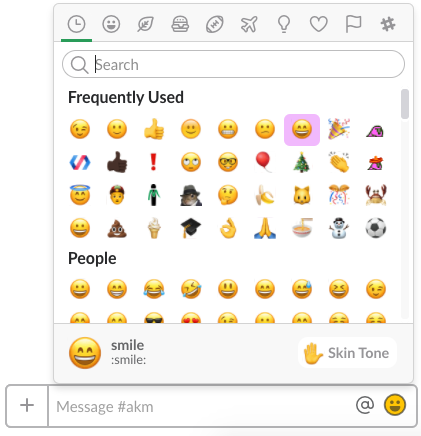
\includegraphics[width=\textwidth]{emojipasswords/slack-picker-shortcode}
	\caption{\label{fig:emojipasswords:slack-picker} The picker shows the short-code of the emoji for future use.}
	\end{subfigure}
	\begin{subfigure}[t]{0.49\textwidth}
	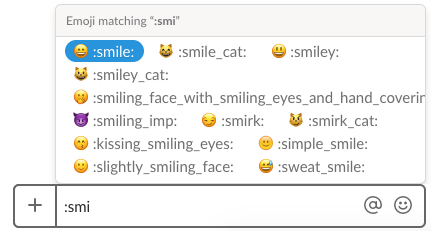
\includegraphics[width=\textwidth]{emojipasswords/slack-shortcode-auto}
	\caption{\label{fig:emojipasswords:slack-picker-shortcode} The user can guess the shortcode. Slack offers matching emojis.}
	\end{subfigure}
	\caption{\label{fig:emojipasswords:slack-emoji-interaction}
		Slack allows the user to utilize both a point-and-click interface and shortcodes to enter emoijs.
	} 
\end{figure}


\subsection{Password Selection in the Lab}
For the first part, participants were invited to a lab at the media informatics research group. The primary task was to create a password that participants could remember well. There was no independent variable for the password selection task, thus participants all received the same study instructions. 

\subsubsection{Metrics}
% no clear-text passwords, emojis and zxcvbn stats, hashes are stored for verification purposes.
We logged the chosen emojis and their positions inside the passwords. Moreover, we analyzed password characteristics with zxcvbn and stored this to the database along with the hashed password. 
% time
As an indicator for usability of either the picker or the shortcodes, we measured the time taken to select the password. Here, we used the ``focus'' and ``blur'' events as start and end points. 

% self-reported: (questionnaire) selection strategies, motivation, input type (motivation, ease of use, usefulness, 5 point scale)
On the qualitative side, we used ordinal five-point scales to collect attitudinal data about using emojis inside passwords, the picker, and shortcodes. Demographic data and self-reported password behavior helped us put measurements into context. 
% think aloud protocol, exit interview.
Everything that participants said during the study was protocolled. 

\subsubsection{Procedure}
% PC self guided with aid of experimenter
% briefing and informed consent (log data will be generated from interactions).
After an in-depth briefing on the purpose of the study and data collection practices, an experimenter explained each step of the study. We provided a standard desktop PC to complete the tasks, which were mostly self-guided. First, participants created a user ID. 
% create user Id (algorithm first letter parents' namses, birthplace, birth month)
Since they were going to need this ID later on to allow us matching the lab and field data, we provided a simple algorithm to create an ID. Participants were asked to take the first letter of both their parents' first names and their own birth place, appended by the digit of their birth month (e.g. ``IKP10''). This algorithm, albeit not perfectly random, was sufficient to protect \acrlong{PII}.

This was followed by a questionnaire on demographic data, password coping strategies and attitudes towards emojis in passwords, e.g. ``\textit{how likely would you consider using emojis in a password?}'' At this point of the study, participants had not yet created an emoji-password, so their attitudes were not biased by the tasks that followed. 
% instruction: difference between emojis and emoticons (shared understanding)
We also briefed them about the difference between ``emojis'' and ``emoticons'' to avoid misinterpretation. 

% password selection & commitment (think aloud)
% scenario: whatsapp requires all users to secure their account with a password (basic8 + emoji, feedback provided when policy is met.) 
Afterwards, participants completed the password selection task using the prototype. A significant part of the screen was dedicated to list all emojis and their short codes. To provide sufficient background information and introduce a realistic risk \cite{Krol2016ExperimentDesign}, the task included a scenario. It asked participants to imagine that they had used WhatsApp for some time and now a new security precaution is introduced. As a safety measure, they were now required to prove their identity with a password upon activating WhatsApp on a new device. The password needed to consist of at least eight alphanumeric characters and at least one emoji. 
% repeat password, only proceed if confirmed to have memorized the password.
Participants then had to repeat the selected password, and tick a box to confirm that they had memorized it (see Figure \ref{fig:emojipasswords:policy-memo-instruction}). 
% usability rating (picker/short codes, emoij-password concept post experience)
This was followed-up through a reflective self-assessment of their behavior during the study (cf. \cite{Fahl2013EcologicalValidityPasswordStudy}), and a structured questionnaire on their selection strategies. 

% interpretation task 
The study concluded with an interpretation task of two given emojis, namely the ``information desk person'' (\emoji{1F481}) and ``folded hands'' (\emoji{1F64F}). Those were not available during password selection, and we intended to assess their suitability for future inclusion. In total, the whole session duration was below 15 minutes.

\begin{figure}
	\centering
	\begin{subfigure}[t]{0.45\textwidth}
		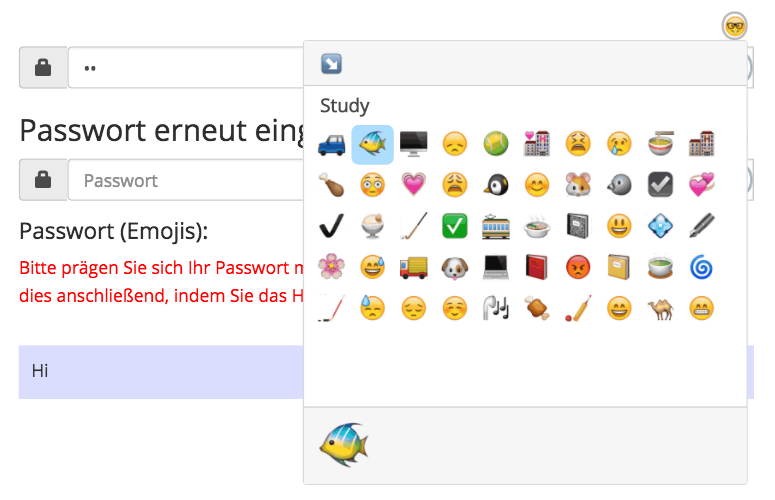
\includegraphics[width=\textwidth]{emojipasswords/open-picker}
		\caption{\label{fig:emojipasswords:ui-open-picker} Point and click interface. It is opened by clicking on the \emoji{1F913} button. The order of emojis is randomized. Upon selecting an emoji, it automatically closes.}
	\end{subfigure}
	\hspace*{0.2cm}
	\begin{subfigure}[t]{0.45\textwidth}
		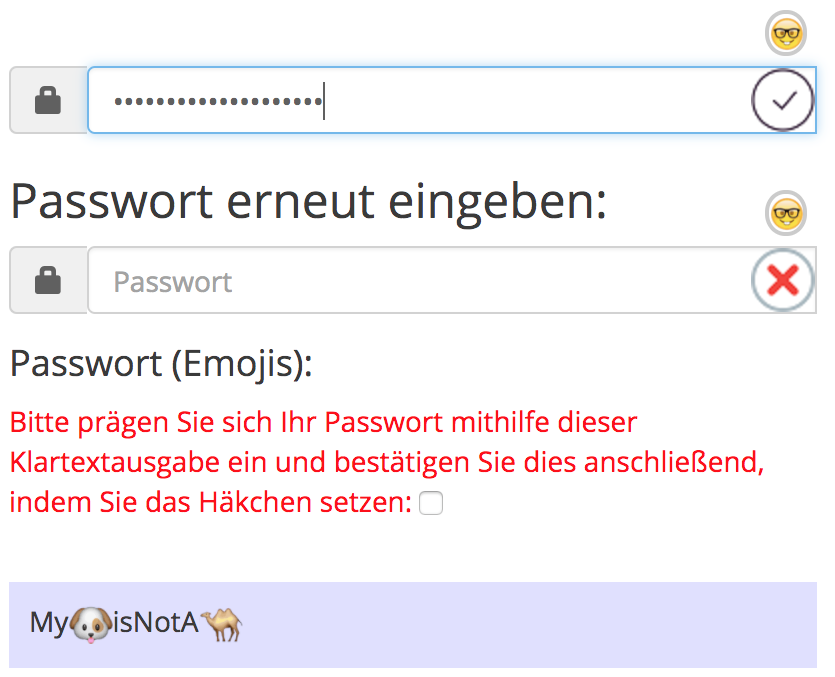
\includegraphics[width=\textwidth]{emojipasswords/ui-slim_cropped-2}
		\caption{\label{fig:emojipasswords:policy-memo-instruction} Screenshot of the user study. The selected password needed to be re-created. Additionally, participants need to tick a check-box to confirm that they had memorized their password.}
	\end{subfigure}
	\caption{\label{fig:emojipasswords:prototype} Prototype as used in the study.}
\end{figure}

% recall
\subsection{Unmoderated Remote Memorability Study}
% exactly one week after participant, invitation to return to the online study. 
Exactly one week after completing the first study part in the lab, participants were invited to return for the second round of tasks on-line. It primarily focused on memorability metrics and a reassessment of attitudes. 
\subsubsection{Independent Variable}
% emoji rendering (2 levels / degrees of freedom ): control group received iOS 9.3 (the same kind as in the lab), experimental group different treatment (Androd 7.0). 
To gauge the influence of emoji fragmentation, we used one independent variable \textit{``rendering''} with two levels. For the \textit{control} group, emojis in the picker were rendered as before. In the experimental group, we replaced the iOS emojis with the Android 7.0 version. No other variations were made. 
\subsubsection{Dependent Variables}
% attempts to log in (max 3). 1 = immediate success, no errors.
We measured the number of attempts participants needed to log in. If they failed to log in on the first try, we counted this as an error.  Moreover, we collected memorization and recall techniques. 
% qual: how memorized? attitudinal ratings, qualitative feedback on overall technique
Finally, subjective usability ratings on the overall concept and qualitative feedback were gathered. This part of the study took about five minutes.

\subsubsection{Procedure}
% randomly put into the two treatment groups, different participation link for the two groups via email
Participants were randomly assigned to one of the two experimental groups. We emailed the corresponding link to the online study and requested completion within two days. 
% recreate user id same algorithm as in the lab)
The web page instructed them to recreate their user ID, providing the same algorithm as in the first part. Afterwards, participants were asked to log-in via their previously selected password. After three unsuccessful attempts, the log-in counted as failed and the study proceeded automatically. However, as a memory support tool, we displayed the list of short codes after the first failed attempts. The study concluded with an attitudinal questionnaire about the perceived usability of the concept. 

\subsection{Recruiting and Demography}
We spread a registration link for a ``study on emojis'' via social networks and an official university newsletter. A 5€ shopping voucher served as incentive. The study was announced to take around 15 minutes. 40 people were screened in and all showed up to their study appointment. All of them were students at the LMU, and aged between 19 and 44 ($M=23$).  %TODO add standard deviation. (if we have it)
Users in this age rage are most likely to use emojis on a regular basis \cite{EmogiResearch2016}. 39 participants returned for the second study part on-line. The control group was formed by 20 participants, and the experimental group by 19. 
%TODO maybe add hypotheses, but that's not super necessary
\section{Results}
In the following, we explain participants' sentiment regarding the usage of emoji-passwords before we report empirical observations and qualitative analyses. 
\subsection{Sentiment}
Sentiments were assessed with agreement levels to five-point scale items (1 = strongly disagree, 5 = strongly agree).
%before.
Before participants selected an emoji-password for the first time, they were already reserved towards the statement ``I would consider adding an emoji to a password'' ($M=2.7, SD = 1.4, Md=2$). They did not regard emojis as a way to make passwords more memorable, either ($M=2.8, SD = 1.3, Md=3$).
%after first trial
After completing the first part, the statement ``I liked adding an emoji to my password'' was rated slightly more positively with an average of 3.6 ($SD=1.19, Md=4$). 
%final sentiment.
Having fulfilled all tasks, participants saw general benefits to add emojis in passwords ($M=3.5, SD = 1.2, Md=4$). Eleven found the enforced emoji-policy annoying. Hence, attitudes towards using emojis for their personal passwords in the future were rather negative ($M=2.6, SD = 1.3, Md=2$), although they were slightly more positive about potential memorability benefits than before ($M=3.1, SD = 1.3, Md=3$). In summary, participants were reserved towards adopting emoji-passwords, but their sentiment covered the full spectrum. 

\subsection{Emoji Selection}
% quant:
% 	which emoijs were selected (distribution graph like on slides)
% 	position in password -> new graph (R!), with data from slides.
\subsubsection{Statistics}
Our 40 participants chose a total of 22 different emojis. Most commonly, participants chose the camel (:camel: \emoji{1F42B}, n=5), penguin (:penguin: \emoji{1F427}, n=5), grinning face (:grin: \emoji{1F601}, n=3), tea (:tea: \emoji{1F375}, n=3), dog (:dog: \emoji{1F436}, n=3), diamond (:diamond\_shape\_with\_a\_dot\_inside: \emoji{1F4A0}, n=3), and cherry blossom (:cherry\_blossom: \emoji{1F338}, n=3). The remaining 15 emojis were chosen less than three times each. Six participants added two emojis to their password though this was not required. On average, password fields had focus for 52.9 seconds ($SD = 55.00$).

\begin{figure}
	\centering
	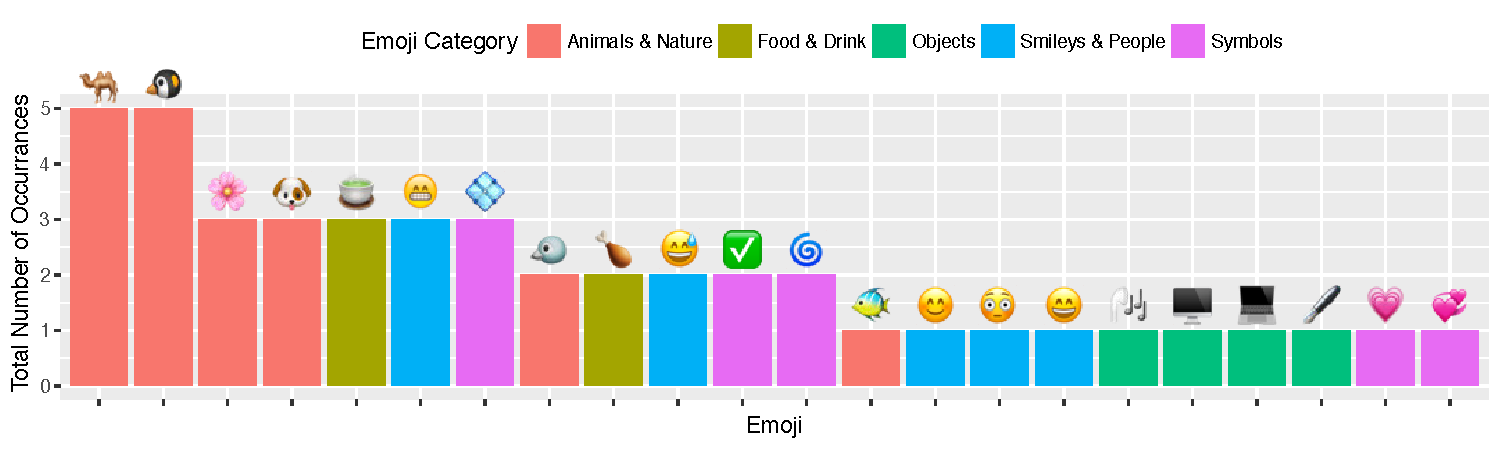
\includegraphics[width=\linewidth]{figures/emojipasswords/emoji-distribution-histogram}
	\caption{\label{fig:emojipasswords:distribution-histogram} Histogram of the chosen emojis and their categories. Patterns emerge already in our sample with 40 participants, which hints at potential security problems.}
\end{figure}


Before passwords were hashed, we determined the position of the emojis. The majority of participants who only selected one emoji put it at the end ($n=19$), while seven started with it and eight put it somewhere in the middle. Adding the emoji there is the most cumbersome approach due to the double modality switch between mouse and keyboard if the picker is used. The six participants who picked two emojis either put both at the start ($n=1$), as the first and last characters ($n=2$), only in the middle as two consecutive characters ($n=1$), or as middle and last character ($n=2$). Figure \ref{fig:emojipasswords:position-histogram-by-strategy} shows a detailed breakdown of the chosen positions. 
\begin{figure}
	\centering
	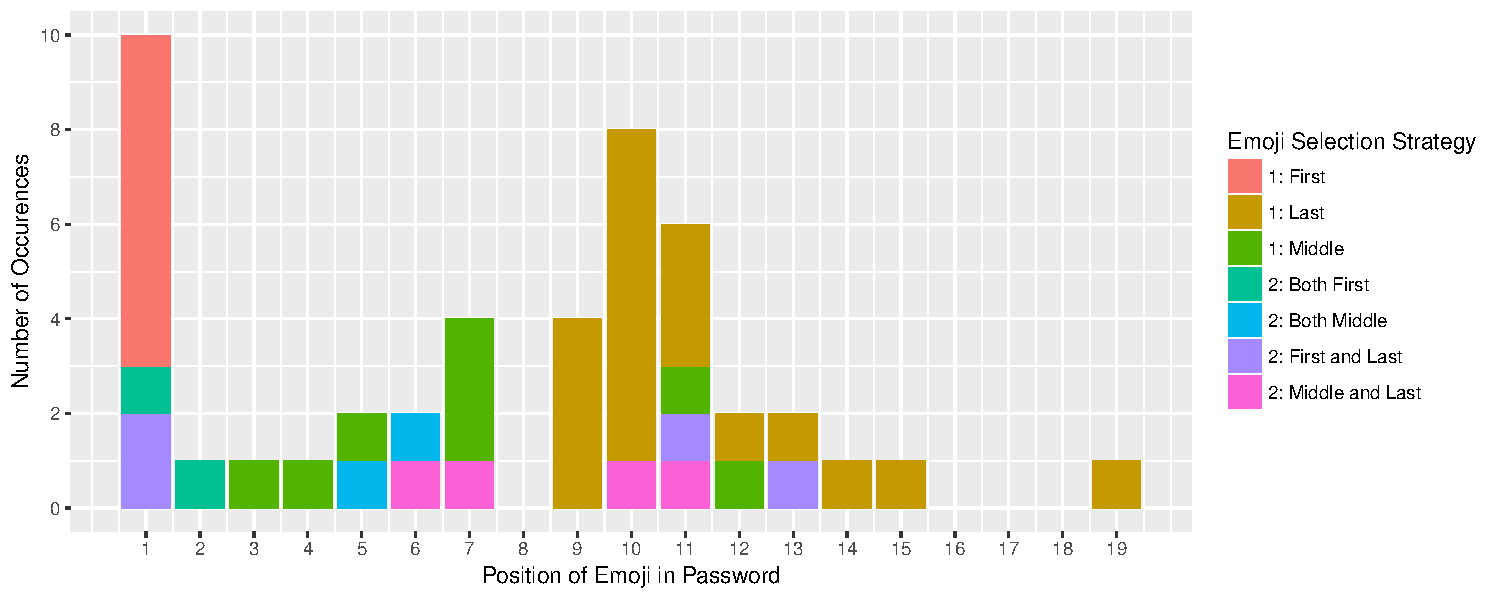
\includegraphics[width=\linewidth]{emojipasswords/position-histogram-by-strategy}
	\caption{\label{fig:emojipasswords:position-histogram-by-strategy} Histogram of absolute positions of emojis inside passwords. The prefix (1:, 2:) denotes the total number of emojis in the corresponding password. Most participants either started or finished their password with the emoji.}
\end{figure}


\subsubsection{Self-Reported Selection Strategies}
Apart from the emoji, our participants mostly claimed to have created a password like they normally would ($M=3.4, SD=1.45, Md=4$). 
% 	selection strategies
We elicited selection strategies in two ways: a list of probable strategies that we identified in pre-tests, and an open question where participants were asked to describe their method in detail. Half of the participants indicated that they used an emoji that fits the alphanumeric part of the password. Four said that they preferred an emoji that they frequently use, while another four chose an emoji at random. The remaining participants either associated the picture to a life event ($n=3$) or hobby ($n=1$). Eight participants elaborated on their tactics in high detail, and their strategies were more individual than the predefined categories. 

Through collaborative thematic analysis, a method similar to affinity diagramming, we identified themes in all qualitative statements and the think-aloud protocol. After the first round of coding, there were 42 codes that were further reduced in an axial coding step. The resulting overall themes were:
\begin{itemize}[leftmargin=*]
	\item \textbf{Internal consistency:} The emoji semantically matches the alphanumeric part of the password, e.g. putting a camel emoji \emoji{1F42B} after the Greek word for ``heat'' (P26). 
	\item \textbf{Context cues:} The password contains a hint to the participant's location or to its purpose. For instance, participants used the computer emoji \emoji{1F5A5} because they created the password on a PC (P34). Another participant picked the check mark \emoji{2705} because it stands for \textit{completing} the study (P38). 
	\item \textbf{Replacement:} The emoji replaces either a letter or an entire word. For instance, P17 replaced the letter ``p'' in their password with a penguin \emoji{1F427} because both \textit{words} begin with the same letter.
	\item \textbf{Appeal:} The emoji visually or emotionally appealed to the participants (mentioned twice for the flower emoji \emoji{1F338})
	\item \textbf{Liking:} Participants had an affection or personal connection to the emoji, e.g. penguins \emoji{1F427}.
	\item \textbf{Usability and Security:} An emoji that serves to increase usability or security of the password. Usability could be improved either with a particularly easy-to-type shortcode (:grin:), or by choosing emojis that ``stand out from the rest, because they look too similar'' (P32, chose the penguin). Security was achieved through perceived randomness or unpredictability (mentioned twice for the diamond \emoji{1F4A0}).
\end{itemize}

Within those six themes, we can see a common story line: The selection strategies can be read as an attempt to \textbf{improve memorability} of the password. Most participants intuitively focused on creating a password that they could easily recall. None of them mentioned the option to write down the emoji-password or store it externally. The selected emojis thus matched individual memorization approaches.

\subsection{Input Methods}
% quant: 
% 	how many used what
The majority ($n=32$) intuitively turned to the point-and-click interface to enter their emoji. Five participants used the short-codes and three tried both modalities. Both the picker and the short codes received positive usability ratings from the respective participants ($M_{picker})=3.8, SD_{picker}=1.1, M_{short}=4.2, SD_{short}=1.3$),  Thus, it was easy for participants to enter emojis on a desktop computer in both modalities. Interestingly, the three participants who tried both methods started with the picker and then continued to use the short codes, because they found it more convenient.

% qual:
%	why? feedback, sentiment.
Through a qualitative analysis of the think aloud protocol we found that participants considered the advantages and disadvantages of both input methods. The picker was perceived as easy and fast to use, while being less prone to typing errors. Often, participants mentioned that they were already familiar with this entry method (e.g. from WhatsApp web), so they did not have to learn anything new. On the other hand, they described the progressive disclosure paradigm as potential problem, because the button that triggers the picker could be overlooked. Also, some mentioned that it is cumbersome to switch between mouse and keyboard. Those who used the shortcodes appreciated the speed of entry and low effort to add the emoji to the password. However, learning and memorizing the corresponding codes were seen as the main drawbacks. The sentiments did not significantly change in the second part of the study ($M=3.5, SD=1.2, Md=4$, overall happiness ratings). In summary, we can conclude that participants made a deliberate choice about the chosen input method and they were happy with it. %TODO add likert plot.

\subsection{Memorability and Recognition}
% quant: 
%	how many succeeded? which emojis were involved in errors? group differences
% 	show the differences visually (like google talk)
\subsubsection{Success Rates}
Login success rates in the second session did not significantly differ between the two study groups. In the control group, who saw the identical emoji set, five participants failed to log in after a week and 15 succeeded. The experimental group, who received the Android version of the emojis, counted six log-in failures, while 13 participants were able to authenticate despite the change of rendering. This difference was not statistically significant ($\chi^2(1)=0.21, p>0.5$). From those who succeeded, 12 participants authenticated on the first try in the control group, whereas this number was slightly lower in the experimental group ($n=8$). Again, the change was not statistically significant ($\chi^2(1)=1.25, p>0.1$), which is probably owed to the sample size. The medians of failed attempts, which are potentially more descriptive in this situation, did differ: the control group's median was 0, while it was 1 in the experimental group. Figure \ref{fig:emojipasswords:success-vs-failures} visualizes successful and unsuccessful login attempts in high detail. There, we can trace back the emoji that were included in incorrectly entered passwords. Success and failure rates in the ``Animals \& Nature'' category were balanced in both groups. However, participants were twice as likely to fail in the experimental group, if their password contained an emoji from the ``Smileys \& People'' category. Figure \ref{fig:emojipasswords:experimental-group-failures} shows that emojis differing strongly from the iOS version were more associated with login failures. ``Symbols'' were the category with the highest failure rate across both groups.


\begin{figure}
	\centering
	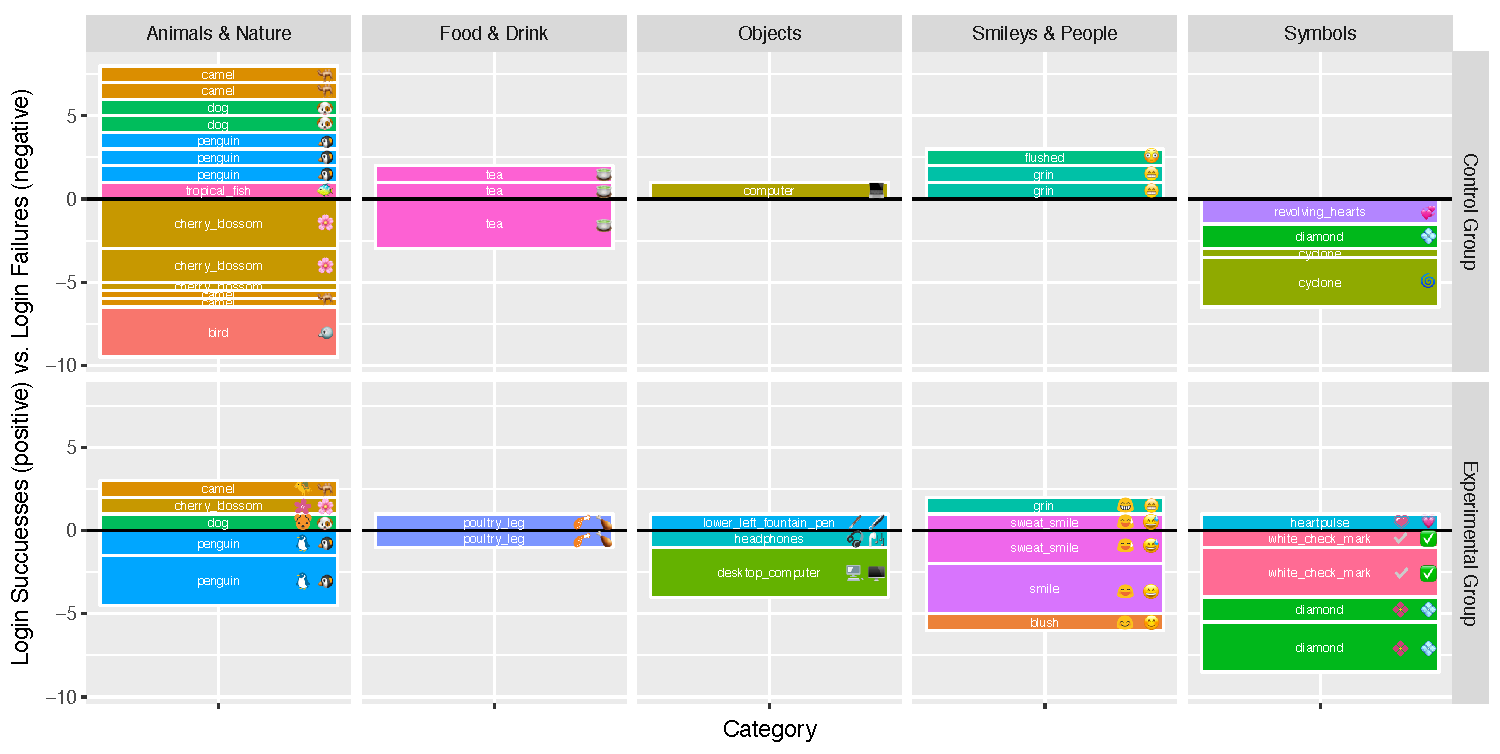
\includegraphics[width=\linewidth]{figures/emojipasswords/success-vs-failures}
	\caption{
		\label{fig:emojipasswords:success-vs-failures}
		Detailed overview of the emojis inside passwords. Columns represent emoji category. The top half shows the control group's attempts while the bottom depicts the experimental group who had to log in with a different emoji style. Successful logins appear on the positive side of the y-axis, and erroneous login attempts on the negative side. Smileys \& People are error prone in the experimental group. Symbols generally led to more errors. 
	}
\end{figure}

\begin{figure}
	\centering
	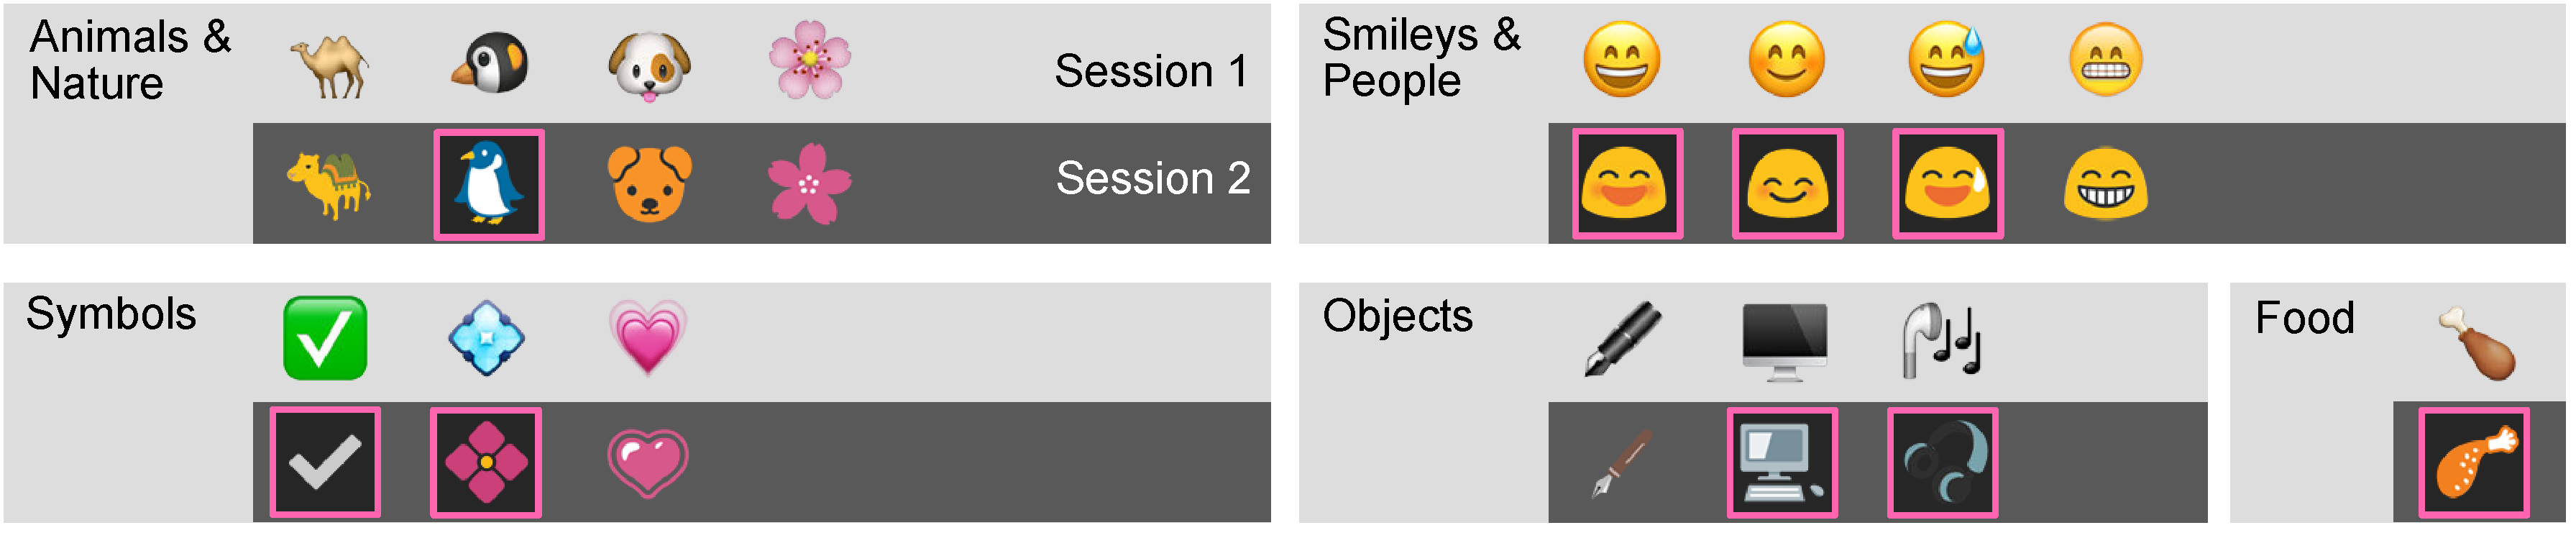
\includegraphics[width=\linewidth]{figures/emojipasswords/experimental-group-errors}
	\caption{
		\label{fig:emojipasswords:experimental-group-failures}
		Effective emoji-set of the experimental group. Error-prone emojis are highlighted with a pink outline. We can see that these differ strongly from the iOS version from session 1. We take this as evidence for the usability problems caused by fragmentation.
	}
\end{figure}


\subsubsection{Textual Feedback}
%	noticed differences?
To assess the influence of the rendering modification, we asked whether participants had noticed any differences in the appearance of the emoji. Although the emojis remained identical in the control group, 7 out of the 20 participants indicated that they had noticed a change. This is hard to interpret, but we assume that they meant the order of the emoji inside the 10x5 grid. In the experimental group, where emojis did in fact \textit{look} different, 16 out of 19 participants (84\%) talked about this change in the response field. Eight of them did not perceive the alteration as troublesome, while another eight felt that identifying the right emoji was challenging. For three participants, the change of emoji-type was insurmountable: One participant was very sure to have selected the correct emoji, because she picked a ``happy face'' to express herself. However, she reported to have failed because she was unable to pick the correct emoji in the second study session. Another participant, who successfully authenticated with his emoji-password, indicated that he could only find the right emoji after a Google search. Finally, one participant mentioned that he was troubled by the different versions of the check mark, so he used a trial and error approach until he succeeded.

\subsection{Memorization Techniques}
%	how did people remember? memorization strategies
%	was the short code useful?
The emoji-picker and the number of emojis was helpful to recognize and recall the password for 18 participants. The short codes did not achieve this, because only one person reportedly used the code as a cue to the password. A priori agreement levels to the statement ``Using emojis in a password makes it more memorable'' were neutral with a tendency to disagreement ($M=2.8, SD=1.4, Md=2$). In the exit survey, we again probed this sentiment and noticed a small, statistically insignificant upward trend ($M=3.1, SD=1.3, Md=$\textbf{3}). 

\subsection{Interpretation Task}
% basically what we wrote in the paper to illustrate that already for two given emojis there is a huge range of possible interpretations.
The final task in the lab-session was to provide two word associations for two emojis (\emoji{1F481}, \emoji{1F64F}). Thematic analyses showed a wide range of themes for the ``service person'' emoji. A total of 14 distinct themes were visible, each mentioned by at least two participants. Most often, this emoji was associated with ``female'' ($n=6$) and ``pointing'' ($n=5$). The emoji depicts a bell-hop's ``tipping gesture'', which was interpreted as ``sassy'' ($n=2$) or ``bossy'' ($n=4$), too. Regarding the ``praying hands'' emoji, participants reached higher consensus on its meaning. Seven themes emerged from the word associations. Most commonly, the participants mentioned ``pray'' ($n=19$) and ``beg'' ($n=9$). These anecdotal examples highlight the problems produced by unclear meanings of emojis. For passwords, on the other hand, a bigger range of interpretations opens up more opportunities to create a story with emojis.

\subsection{Limitations}
% small sample size, homogeneous --> primary user group who are most likely to adopt emojipws as first-movers.
The results presented above need to be interpreted in the light of a few important limitations. First, the \textbf{sample size} was not large enough to bring about statistically significant test results. Naturally, the null hypotheses (e.g. fragmentation does not affect recall) could be true, but with 40 participants, we lack some statistical power to draw conclusive inferences, especially with a frequentist approach (which emoji was chosen \textit{how often}). Nevertheless, we saw emerging patterns that can be followed up with a quantitative user study. Our primary goal was the exploration of fragmentation and input issues, as well as attitudes. Our participants belonged to the user group who would be most likely to try out emoji-passwords. This makes us confident the trends at least point into the right direction. To explore additional dimensions of the problem space around emoji-passwords, considering a more diverse sample is going to be useful in the future.

% ecological validity, self-report, novelty effects --> concrete plausible scenario, no reason not to trust P's.
Moreover, much of the elicited data is attitudinal, potentially affecting ecological validity of the study. However, we tried to mitigate issues by providing a realistic scenario and had them gauge their behavior. Here, most claimed they acted like they normally would, which has been shown to be a useful indicator as to the trustworthiness of the data \cite{Fahl2013EcologicalValidityPasswordStudy}. Nonetheless, emoji-passwords constituted an unfamiliar paradigm for all participants, despite their familiarity with both emojis and passwords separately. Therefore, novelty effects are possible in that participants might have spent more time to explore the possibilities than they normally would. However, subjective usability assessments on the feasibility of emoji-passwords were reserved nonetheless. This indicates that respondents critically balanced the pros and cons and did not only focus on the benefits.

% no attack vectors, only usability, behavioral, attitudinal data --> future work, but maybe compare to the advantage of adding a Xclass requirement over X-1class requirement from another study. that should do. 
% no full-factorial design. 

\section{Discussion}
In the following, the results are put into context. We derive data-driven assessments about the feasibility of emoji-passwords. 
\subsection{Selection Strategies and Their Implications}
% what did they focus on? --> memorability, not security
% what does that mean?
% does that help?
% covariate: personality? \cite{Marengo2017EmojiPersonality}
% central point: focus on memorability, not security.
It was evident that participants were keen on creating a \textbf{memorable password}. So although people were enabled to select a richer and more diverse password, we observed well-known reactions. 
% selection strategies are just like they used to be, i.e. bad.
The selection strategies were a direct translation of their usual patterns. Many of them noted that they were able to easily include emojis in their long-established strategies and coping behavior. As a consequence, we observed predictable patterns in selection strategies leading to simple attack vectors: participants favored items that helped them maintain their existing selection strategies, which can be exploited to adapt cracking techniques.
% what does that mean? all bad?
We can read this as a bad sign, because emojis do not appear to break existing behavior, and only increase the theoretical space of creation strategies. At this point it is difficult to gauge practical security advantages entailed by enlarging the character set. Learning from past roll-outs of new authentication schemes, password \textit{strength} is unlikely to increase drastically by the use of emojis. 
% it's not going to get worse, security wise. so we got that going for us.
On the other hand, user-selected passwords have always shown predictable patterns and adding emojis probably will not aggravate the situation further. Therefore, the only major advantage of allowing users to pick emoji-passwords can be an improvement in how password authentication is perceived. In other words, it might help the \textbf{\gls{UX}}. Our data is helpful to identify the pitfalls that need to be considered to achieve good UX of emoji-passwords. 

\subsection{Factors in Good UX of Emoji Passwords}
Improving the UX of a technology is a strategy to drive its persuasiveness \cite{Fogg2001WhatMakesSitesCredible}. Therefore, we can address a number of aspects to foster a positive user experience of emoji-passwords.  
% freedom to choose. not everyone likes that. large spectrum of ratings, median: neutral!
\paragraph{Freedom to choose} Good UX starts with respect and empathy. Users should not be forced to use emojis in their passwords. Our data discourages the use of a policy that mandates emojis, which a quarter of participants found annoying. Our first study on personality factors showed a large variety of thinking styles about policies (cf. Section \ref{sec:personality:study-1}). Therefore, we argue in favor of autonomy and leaving it up to users to decide whether they want to use an emoji as part of their password(s). So, users are \textit{empowered} to change their behavior and might be persuaded to do so. 

% IF users understand that they can use emoji-passwords, doing so needs to be frictionless and it is no problem to achieve this.
\paragraph{Learning Curve} Once users understand that they have the freedom to use emoji-passwords, the learning curve for this task looks fairly gentle. Our sample consisted of users who were already familiar with entering emojis on the desktop and therefore immediately knew what to do. Less experienced user groups should be offered assistance in case they decide to experiment with emoji-passwords. We also found that the short codes were mainly used by participants who aimed for efficiency. Thus, there is nothing wrong with enabling short codes for input, but it should be tailored to an advanced user group. 

%- don't have to learn anything new: emojis are familiar, interaction is familiar (shortcodes maybe for experts),

% rendering
\paragraph{Pragmatic Constraints for Passwords}\label{sec:emojipasswords:unique-constraints} 
%yo! stick to the same kind of emojis. be smart. whatsapp also has the same emojis on all platforms. but interference effects of using different platforms with different emoji-passwords are likely to arise. 

% fragmentation nono, consistency yes yes.
Although our sample came from a population of young adults who are highly experienced with emojis, some participants clearly struggled to identify the correct emoji after we exchanged the renderings. Therefore, inconsistencies across platforms could become a show-stopper. At the moment, there are a few problems that contribute to creating inconsistent experiences. 
% challenges: legal / copyright
First, although emojis are standardized Unicode \textit{code-points}, vendors usually need to create custom emoji-\textit{pictures} for legal reasons. Sets under a public domain or nonrestrictive licenses do exist, but many vendors prefer shipping custom on-brand experiences with a shared design language across their products. On the other hand, it could be useful to form alliances like the \gls{W3C} to standardize graphical assets of emojis specifically for password-fields. Software keyboards on mobiles would also need to match this hypothetical ``password-emoji standard''. As of now, emojis offered by built-in software keyboards often look different to those of certain apps (see Figure \ref{fig:emojipasswords.app-vs-platform-emojis}). To solve this inconsistency, a native keyboard could offer an interface that lets the app inject a consistent set of emojis.

% challenges: distinctiveness
After settling on a shared visual representation of emojis, distinctiveness is another critical factor. Some emoji-tuples that look very similar to each other can be troublesome. One of our participants mentioned this issue already in his selection strategy, because he was looking for an emoji that ``stands out'' and did not ``look like the others''. To avoid login failures from confusion, there needs to be a whitelist of emojis that only contains the highly distinctive ones. We can first derive a candidate list based on geometric parameters like shape and color, and then proceed to evaluate them through quantitative user research with a diverse sample.

% challenges: reduction?
A final challenge pertaining to the constraints of emoji-passwords are hard usability metrics like efficiency. Higher degree of freedom and creativity support are ineffective if users need to browse through large lists of emojis only to find the correct item. Reducing the emoji-space to a subset emerges as a useful approach to speed up recognition and efficiency. At the same time, it is conceivable that vendors stick to a limited, static subset that is randomly selected from the whitelist of distinct emojis. Distinct subsets, i.e. a different random permutation per vendor, can also mitigate password reuse. 

\begin{figure}
	\centering
	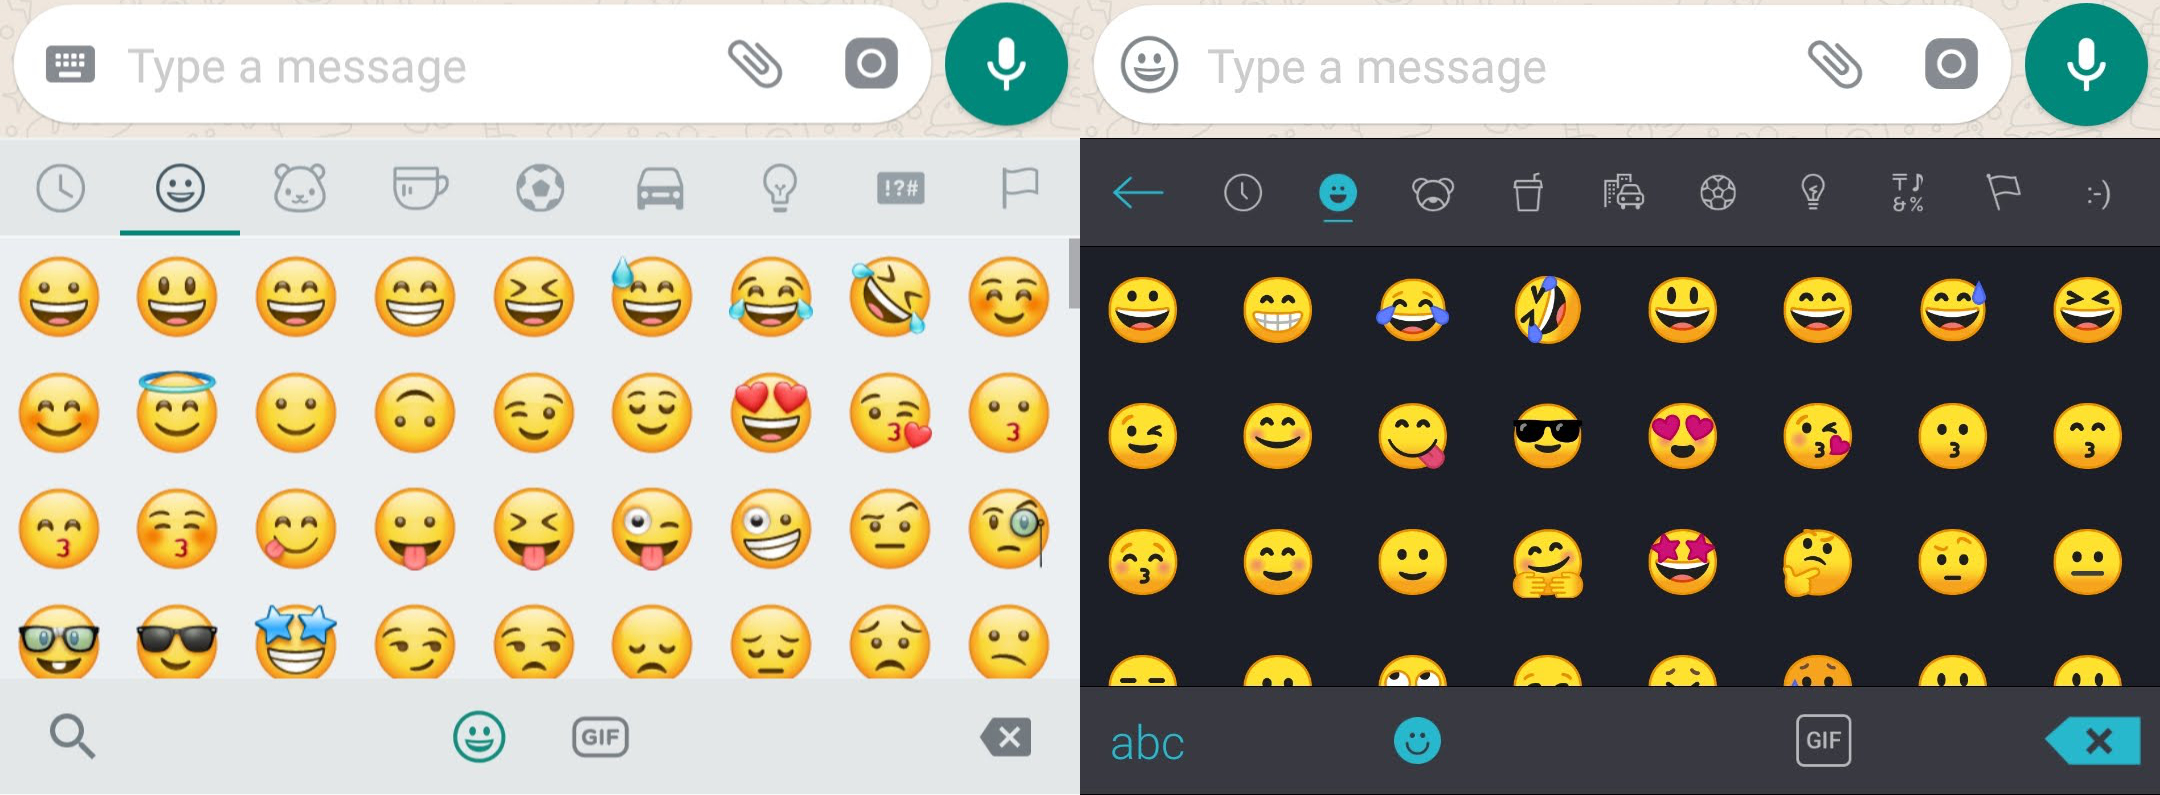
\includegraphics[width=0.7\linewidth]{figures/emojipasswords/app-vs-platform-emojis}
	\caption{\label{fig:emojipasswords.app-vs-platform-emojis}
		Screenshots of entering emojis on WhatsApp. While the software provides a set of emojis that is consistent across all platforms supported by WhatsApp (left), users can still turn to the native software keyboard of their OS (right). In this case, the renderings, number, and order are inconsistent.
	}
\end{figure}



%\subsection{Similarity and Fragmentation Issues}
% not yet crystal clea

% from the paper: While three comments pointed towards a different interpretation, the numbers suggest that the different renderings of emojis did not have a notable impact on the login success rates, i.e. reproducibility of the emoji-passwords. The small sample size increases the likelihood of type-2 for statistical tests, though. In that case, this would explain the low voluntary readiness to include emojis in their personal passwords. Nonetheless, qualitative evidence is conclusive that users try to leverage emojis for creating more memorable secrets, if the emojis are required by the password policy.


%\subsection{Input UX}
% was it troubling? no
% does that mean, that all password fields on desktops should be accompanied by 
% of course entering an emojipw takes longer. even reading a text that includes emoji takes longer \cite{Gustafsson2017EmojiReadingTIme}


\section{Conclusion}
% summary and answers to research questions.
In this project, we empirically evaluated the usage of emojis in regular alphanumeric passwords to gauge their suitability as persuasive alternative to existing passwords. Our mixed-model user study with forty participants focused on attitudinal and usability aspects. From the selection behavior, memorability results and qualitative feedback we can conclude that emojis do not necessarily lead to memorable passwords (RQ1). Participants wanted to translate their usual password selection behavior to the new paradigm and at least tried to create memorable passwords (RQ4). When participants failed to log in, this could be partially traced back to fragmentation, i.e. differences in the visual representation of the same emoji characters (RQ2). Our sample population was experienced with emojis, but still struggled to match Android emojis to a previously selected iOS emoji. Their personal experience allowed them to easily understand how to enter emoji-passwords on desktops through a graphical point-and-click interface (RQ3). Nevertheless, our prototype made potential usability problems salient for participants and thus their attitudes towards adopting emoji-passwords in the future were reserved (RQ5). Thus, the persuasive power of emoji-passwords was limited, which we attribute to the user experience of the study setting. 

% motivate / show the big picture of why our answers matter now. 
Some vendors and service providers have already enabled emoji support for passwords. For instance, Twitter\footurl{https://www.twitter.com}{10.03.2018} allows users to take advantage of this rich character set. The issues we explored in our study thus affect a growing number of users already now. Roadmaps to address fragmentation and input issues do not exist at this point. However, more and more users are going to find out about the capabilities, perhaps because the feature is presented in blog- and news articles \cite{Dashinsky2015NoEmojisInPWs}. Therefore, the HCI community should act quick to create a better authentication experience to \textbf{scale solutions before problems are going to scale}. 
% lets stay realistic.
Realistically, the propositions and requirements discussed in Section \ref{sec:emojipasswords:unique-constraints} would require intensive negotiation substantiated with much more user testing data.  It is unclear whether vendors are willing to make this investment. We argue that a standardized \textit{emoji-password-picker} with a random sub-set of white-listed, distinctive emojis is a desirable goal. The ``longer term solutions'' that are part of the Unicode standard (see Footnote \ref{foot:emoji-standard}) embrace ``embedded graphics'', which paves the way to mitigate fragmentation issues. Since leading tech companies have worked together on the standardization of emojis in the past, it would be fruitful to collaborate on authentication issues of emojis, too.

\paragraph{Future Work}
% focus on ux
Our prototype did not deliver the best possible user experience. This caveat was partially owed to isolating confounding factors. For instance, a finished solution would not shuffle the order of emojis as we did. Future studies on emoji-passwords need to intensely study different dimensions of user experience issues and potentials. To better understand the current state of emoji-passwords, a diary study might be worthwhile. It would be possible to answer interesting questions on how this novel kind of authentication influences well-established coping strategies. For instance, is it possible to \textbf{write down emoji-passwords}, and \textbf{share} them with somebody else? Can \textbf{password managers} already handle them?  Do users take more care to protect emoji-passwords from \textbf{shoulder surfers}? Such questions can further help judge the feasibility of this approach and identify important pain points.

% quantify security beneftis and provide solutions. 
At the same time, we saw how existing coping strategies might lead to weak emoji-passwords. Therefore, as a next step, the security benefits should be quantified. Perhaps, this is relatively easy to do with an \gls{mTurk} study. If our hunch about weak selection strategies is confirmed, persuasive strength feedback for emoji-passwords is an important future research direction. Real-time password meters, particularly those based on zxcvbn, are currently unable to realistically gauge the strength of emoji-passwords. Therefore, further work on modeling strength is necessary. Neural networks, as shown by Melicher \etal, could respect the predictability of user-chosen emojis in guess-number estimates \cite{Melicher2016NeuralNetworks}. All in all, some more work is going to be necessary to reach the high persuasive power of emoji-passwords that we had hoped for. Our work has laid the foundations for such studies on the quantitative side. 

%\vspace*{2cm}
\pagebreak
\noindent
\fbox{
	\hspace{1cm}
	\parbox[c][12cm]{0.7\linewidth}{
		\section*{Take Aways}
		\begin{itemize}[leftmargin=*]
			\item Users' intuitive reaction to creating an emoji-password was resorting to established strategies with memorability in mind. This is early evidence that the envisioned security benefits might come off very small.
			\item Emojis did not significantly improve password memorability.
			\item Simulating log-ins on a different platform than where the emoji-password was selected resulted in notable usability issues, because users fail to recognize the previously selected emojis.
			\item A point-and-click interface works for emoji-passwords, but emojis must be reduced to a small sample and must not look very similar to each other. 
			\item Most participants were not eager to adapt emoji-passwords. The current user experience reduced the persuasive effects of empowering users to become more creative. % But those eager to use them are likely to face the troubles we identified in our study. 
		\end{itemize}
	}
	\hspace{1cm}
}
